\documentclass{article}

\usepackage{amsmath,amsfonts}
\usepackage[margin=3cm]{geometry}

\usepackage{multirow}

\usepackage{hyperref}
\hypersetup{
    colorlinks = true,
    linkcolor  = blue,
    urlcolor   = blue,
    citecolor  = blue
}

\usepackage{longtable}
\usepackage[usenames, dvipsnames]{xcolor}

\usepackage{tikz}

\usepackage{listings}
\lstdefinestyle{pseudo}
{
    keywordstyle = [1]{\normalfont\bfseries},
    keywordstyle = [2]{\normalfont\it},
    keywordstyle = [3]{\normalfont},
    morekeywords = [1]{repeat, for, to, return, if},
    morekeywords = [2]{A, B, N, M, output, accum, count, prev, i, j, k, d, start, end},
    morekeywords = [3]{let},
    morecomment = [l][\color{BrickRed}\it]{//}
}

\title{Solutions for Data Structures and Algorithms Spring 2023 — Problem Sets}
\author{By Dmitriy Okoneshnikov, B22-DSAI-04}

\begin{document}

\maketitle

\section*{Week 11. Problem set}

\begin{enumerate}
    \item Write down \textbf{all} possible topological sortings for the nodes of the following directed graph:

    \begin{center}
    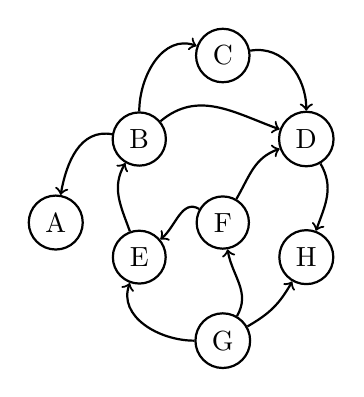
\begin{tikzpicture}[node distance={15mm}, thick, main/.style = {draw, circle}] 

    \node[main] (1) {B};
    \node[main] (2) [below left of=1] {A};
    \node[main] (3) [above right of=1] {C};
    \node[main] (4) [below right of=3] {D};
    \node[main] (5) [below of=4] {H};
    \node[main] (6) [below left of=4] {F};
    \node[main] (7) [below left of=5] {G};
    \node[main] (8) [above left of=7] {E};
    
    \draw[->] (1) to [out=170,in=80,looseness=1.05] (2);
    \draw[->] (1) to [out=90,in=160,looseness=1.05] (3);
    \draw[->] (1) to [out=40,in=160,looseness=1.05] (4);
    \draw[->] (3) to [out=10,in=90,looseness=1.05] (4);
    \draw[->] (4) to [out=300,in=70,looseness=1.05] (5);
    \draw[->] (6) to [out=60,in=200,looseness=1.05] (4);
    \draw[->] (7) to [out=60,in=280,looseness=1.05] (6);
    \draw[->] (7) to [out=30,in=240,looseness=1.05] (5);
    \draw[->] (7) to [out=180,in=250,looseness=1.05] (8);
    \draw[->] (6) to [out=150,in=40,looseness=1.05] (8);
    \draw[->] (8) to [out=110,in=240,looseness=1.05] (1);
    
    \end{tikzpicture}
    \end{center}

    \textbf{Answer.}

    \begin{enumerate}
        \item GFEBCDHA
        \item GFEBCDAH
        \item GFEBCADH
        \item GFEBACDH
    \end{enumerate}

    \item Give an example of a directed graph $G = (V, E)$, a source vertex $s$, and a set of tree edges $T \subseteq E$ such that for each vertex $v \in V$, the unique simple path in the graph $(V, T)$ from $s$ to $v$ is a shortest path in $G$, yet the set of edges $T$ cannot be produced by running BFS on $G$, no matter how the vertices are ordered in each adjacency list.

    \textbf{Answer.}

    The red arrows are part of the tree $T$.

    \begin{center}
    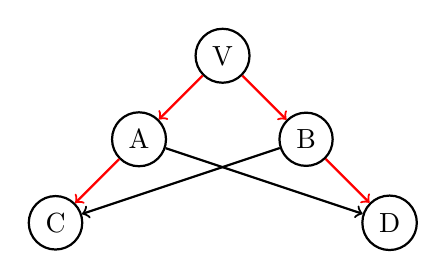
\begin{tikzpicture}[node distance={15mm}, thick, main/.style = {draw, circle}] 

    \node[main] (1) {V};
    \node[main] (2) [below left of=1] {A};
    \node[main] (3) [below right of=1] {B};
    \node[main] (4) [below left of=2] {C};
    \node[main] (5) [below right of=3] {D};

    \draw[red, ->] (1) -- (2);
    \draw[red, ->] (1) -- (3);
    \draw[red, ->] (2) -- (4);
    \draw[red, ->] (3) -- (5);
    \draw[->] (2) -- (5);
    \draw[->] (3) -- (4);
    \end{tikzpicture}
    \end{center}
    
\end{enumerate}


\end{document}
